\documentclass[11pt, dvipsnames, twoside, DIV=12]{scrreprt} %twoside
\usepackage{babel}

%\usepackage{geometry} %showframe

\usepackage[utf8]{inputenc}
\usepackage[T1]{fontenc}
\usepackage{natbib}
\usepackage[nottoc]{tocbibind}
\bibliographystyle{abbrvnat}
\usepackage{subcaption}
\usepackage{booktabs}
\usepackage{multirow}
\usepackage{xurl}
\usepackage[export]{adjustbox}
\usepackage{tabularx}
\usepackage{tabulary}
\usepackage{tikz}
\usepackage{siunitx}
\usepackage[section]{placeins}
\usepackage{multirow}
\usepackage{pdfpages}



\usepackage[multiple]{footmisc}
\usepackage{tablefootnote}
\def\tablefootnotemark#1{\textsuperscript{\getrefnumber{#1}}}

\usetikzlibrary{patterns,decorations.pathreplacing}
\usetikzlibrary{arrows.meta,arrows}
\usetikzlibrary{calc}

\usepackage{paralist}

\usepackage{ifthen}
\newcommand{\CC}[1][]{$\text{C\hspace{-.25ex}}^{_{_{_{++}}}}
\ifthenelse{\equal{#1}{}}{}{\text{\hspace{-.625ex}#1}}$}

\usepackage[usestackEOL]{stackengine}
\usepackage{bm}
\usepackage{amsmath}
\usepackage{amssymb}
\usepackage{amsthm}
\usepackage{amsfonts}
\usepackage{thmtools}		
\usepackage{mleftright}
\usepackage{stmaryrd}
\usepackage{nicefrac}
\usepackage{algorithm}
\usepackage{algorithmicx}
\usepackage[noend]{algpseudocode}
\renewcommand{\algorithmicrequire}{\textbf{Input:}}
\renewcommand{\algorithmicensure}{\textbf{Output:}}
\DeclareMathOperator{\hist}{hist}

\usepackage{dsfont} % For the indicator function: \mathds{1}


% Fixes some spacing issues with braces.
\let\originalleft\left
\let\originalright\right
\renewcommand{\left}{\mathopen{}\mathclose\bgroup\originalleft}
\renewcommand{\right}{\aftergroup\egroup\originalright}

\theoremstyle{definition}
\newtheorem{theorem}{Theorem}
\newtheorem{conjecture}{Conjecture}
\newtheorem{proposition}[theorem]{Proposition}
\newtheorem{insight}{Insight}
\newtheorem{observation}{Observation}
\newtheorem{lemma}[theorem]{Lemma}
\newtheorem{corollary}[theorem]{Corollary}
\newtheorem{definition}[theorem]{Definition}
\newtheorem{example}[theorem]{Example}
\newtheorem{remark}[theorem]{Remark}
\newtheorem{claim}[theorem]{Claim}
\newtheorem{fact}[theorem]{Fact}
\usepackage{thm-restate}
\usepackage[mathic=true]{mathtools}
\usepackage{fixmath}
\usepackage{siunitx}


\usepackage{pifont}
\newcommand{\cmark}{\ding{51}}
\newcommand{\xmark}{\ding{55}}
\usepackage{blindtext}
\usepackage{eso-pic}

\usepackage{xcolor}
\newcommand{\sqbox}[1]{\textcolor{#1}{\rule{1.7ex}{1.7ex}}}

\usepackage{todonotes}

\usepackage{enumitem}
\setlist[enumerate]{itemsep=0.2ex, topsep=0.5\topsep}
\setlist[description]{itemsep=0.2ex, topsep=0.5\topsep}
\setlist[itemize]{itemsep=0.2ex, topsep=0.5\topsep}


% Let cleveref and thmtools work together
\makeatletter
\def\thmt@refnamewithcomma #1#2#3,#4,#5\@nil{%
\@xa\def\csname\thmt@envname #1utorefname\endcsname{#3}%
\ifcsname #2refname\endcsname
\csname #2refname\expandafter\endcsname\expandafter{\thmt@envname}{#3}{#4}%
\fi
}
\makeatother

% Removed 'pagebackref,' as it makes the bilbipgraphy more cluddered in my opinion
\usepackage[
pdfa,
hidelinks,
pdftex, 
pdfdisplaydoctitle,
pdfpagelabels,
pdfauthor={},
pdftitle={},
pdfsubject={},
pdfkeywords={},
pdfproducer={Latex with the hyperref package},
pdfcreator={pdflatex},
hyperfootnotes=true
]{hyperref}

\usepackage[capitalise,noabbrev]{cleveref}   

\usepackage{microtype}
\usepackage{ellipsis}

\usepackage[scaled=0.86]{helvet}
\usepackage{lmodern}

\usepackage{pgfplots}
\usepackage{afterpage}


% Larger sum symbol
\usepackage{graphicx}
\newlength{\depthofsumsign}
\setlength{\depthofsumsign}{\depthof{$\sum$}}
\newlength{\totalheightofsumsign}
\newlength{\heightanddepthofargument}
\newcommand{\nsum}[1][1.4]{% only for \displaystyle
    \mathop{%
        \raisebox
            {-#1\depthofsumsign+1\depthofsumsign}
            {\scalebox
                {#1}
                {$\displaystyle\sum$}%
            }
    }
}

\newcommand{\nnsum}[1][1.2]{% only for \displaystyle
    \mathop{%
        \raisebox
            {-#1\depthofsumsign+1\depthofsumsign}
            {\scalebox
                {#1}
                {$\displaystyle\sum$}%
            }
    }
}

% GNNs
\newcommand{\gat}{\textsf{GAT}\xspace}
\newcommand{\gcn}{\textsf{GCN}\xspace}
\newcommand{\gin}{\textsf{GIN}\xspace}
\newcommand{\gnn}{\textsf{GNN}\xspace}
\newcommand{\gnns}{\textsf{GNN}s\xspace}
\newcommand{\gineeps}{\textsf{GINE-$\varepsilon$}\xspace}

% SI UNIT
\newcommand{\perc}[1]{\SI{#1}{\percent}}

% Bold. 
\newcommand{\mF}{\mathbf{F}}
\newcommand{\mG}{\mathbf{G}}
\newcommand{\mH}{\mathbf{H}}
\newcommand{\mL}{\mathbf{L}}
\newcommand{\mI}{\mathbf{I}}

\newcommand{\mW}{\mathbf{W}}
\newcommand{\ma}{\mathbf{a}}
\newcommand{\mb}{\mathbf{b}}
\newcommand{\mw}{\mathbf{w}}

\newcommand{\ba}{\ensuremath{{\bf a}}}
\newcommand{\bb}{\ensuremath{{\bf b}}}
\newcommand{\bc}{\ensuremath{{\bf c}}}

% Calligraphic.
\newcommand{\cA}{\mathcal{A}}
\newcommand{\cB}{\mathcal{B}}
\newcommand{\cC}{\mathcal{C}}
\newcommand{\cF}{\mathcal{F}}
\newcommand{\cG}{\mathcal{G}}
\newcommand{\cH}{\mathcal{H}}
\newcommand{\cN}{\mathcal{N}}
\newcommand{\cO}{\mathcal{O}}
\newcommand{\cP}{\mathcal{P}}
\newcommand{\cR}{\mathcal{R}}
\newcommand{\cS}{\mathcal{S}}
\newcommand{\cT}{\mathcal{T}}
\newcommand{\cU}{\mathcal{U}}
\newcommand{\cV}{\mathcal{V}}
\newcommand{\cX}{\mathcal{X}}


% Sans serif.
\newcommand{\sC}{\mathsf{C}}

% Blackboard.
\newcommand{\Fb}{\mathbb{F}}
\newcommand{\Gb}{\mathbb{G}}
\newcommand{\Nb}{\mathbb{N}}
\newcommand{\Qb}{\mathbb{Q}}
\newcommand{\Rb}{\mathbb{R}}
\newcommand{\Zb}{\mathbb{Z}}

% Multiset Definition
\newcommand{\MSopen}{\{\!\!\{}
\newcommand{\MSclose}{\}\!\!\}}

% 1-WL+NN
\newcommand{\wlnn}{\text{\textsf{1-WL+NN}}\xspace}
\newcommand{\wliso}{\simeq_{\text{1WL}}}
\newcommand{\knn}{K^{n \times n}}
\newcommand{\gapp}{\textsf{\gnn-Approximating}\xspace}
\newcommand{\wldisc}{\textsf{\wl-Discriminating}\xspace}
\newcommand{\wl}{\textsf{1-WL}\xspace}
\newcommand{\mlp}{\textsf{MLP}\xspace}
\newcommand{\nwl}{n_{\textsf{wl}}}

% Datasets
\newcommand{\enzymes}{\textsc{Enzymes}\xspace}
\newcommand{\nci}{\textsc{Nci1}\xspace}
\newcommand{\mutag}{\textsc{Mutag}\xspace}
\newcommand{\proteins}{\textsc{Proteins}\xspace}
\newcommand{\imdb}{\textsc{Imdb-Binary}\xspace}
\newcommand{\reddit}{\textsc{Reddit-Binary}\xspace}
\newcommand{\zinc}{\textsc{Zinc}\xspace}
\newcommand{\zincten}{\textsc{Zinc(10k)}\xspace}
\newcommand{\alchemy}{\textsc{Alchemy}\xspace}
\newcommand{\alchemyten}{\textsc{Alchemy(10k)}\xspace}

%Parameter for sampling, keep low for fast compile times and increase when submitting the work
\def\samples{5000}


\usepackage[auth-lg]{authblk}
\newcommand{\cm}[1]{{{\textcolor{purple}{\textbf{[CM:} {#1}\textbf{]}}}}}


\renewcommand*{\Affilfont}{\large\normalfont}
\renewcommand*{\Authfont}{\normalfont}

\recalctypearea
\setcounter{Maxaffil}{2}

\title{A Theoretical and Empirical Investigation into the Equivalence of Graph Neural Networks and the Weisfeiler-Leman Algorithm\\
\vspace{20pt}\small{\normalfont From the Faculty of Mathematics, Physics, and Computer Science approved for the purpose of obtaining the academic degree of Bachelor of Sciences.}}
\author{\textbf{Eric Tillmann Bill}}
\affil{\vspace{100pt}}

\author{Supervisor:\\Prof. Dr. rer. nat. Christopher Morris}
\affil{Machine Learning on Graphs Group\\RWTH Aachen University}

\date{\vspace{30pt}August, 2023}

\renewcommand{\thesection}{\thechapter.\arabic{section}}
\numberwithin{equation}{section}
\counterwithout{footnote}{chapter}


\begin{document}
\pagenumbering{Roman}

% % Plotting the logo of the institute in the right corner
% \begin{tikzpicture}[remember picture, overlay]
%     \node[anchor=north east,inner sep=20pt, shift={(-10pt,0)}] (logo) at (current page.north east)
%                {
\includegraphics[scale=0.2]{Figures/rwth_log_en_blau_rgb.png}};
% \end{tikzpicture}
% % Mandatory disclaimer
% {\vspace{5pt}\\\fontfamily{phv}\selectfont \textbf{The present work was submitted to the Machine Learning on Graphs Group at the
% Chair of Computer Science 6, RWTH Aachen University\hspace*{\fill}}}
% % Make title
% {\let\newpage\relax\maketitle}

\includepdf{main_one_sided.pdf}

\begin{table}[H]
	\caption{Overview of the mean absolute error and the standard deviation (logMAE) on large-scale (multi-target) molecular regression tasks. We highlighted the lowest error for the \wlnn and \gnn models for each dataset.}
	\label{tab:results_regression}
	\resizebox{0.975\textwidth}{!}{ 	\renewcommand{\arraystretch}{1.05}
		\begin{tabular}{@{}c <{\enspace}@{}lcccc@{}}	\toprule
			& \multirow{3}{*}{\vspace*{4pt}\textbf{Method}}&\multicolumn{4}{c}{\textbf{Dataset}}
			\\
			\cmidrule{3-6}
			& & {\textsc{Alchemy}} & {\textsc{Alchemy (10k)}} & {\textsc{Zinc}} & {\textsc{Zinc (10k)}} 
			\\	
			\toprule
            & \wlnn & {0.600} {\scriptsize $\pm 0.004$} -0.625 {\scriptsize $\pm 0.032$} & {0.305} {\scriptsize $\pm 0.001$} -1.740 {\scriptsize $\pm 0.042$} & {0.229} {\scriptsize $\pm 0.003$} &	{0.465} {\scriptsize $\pm 0.009$}
			\\
			\cmidrule{2-6}
			& \gnn & {0.523} {\scriptsize $\pm 0.016$} -0.705 {\scriptsize $\pm 0.035$} & {0.282} {\scriptsize $\pm 0.002$} -1.890 {\scriptsize $\pm 0.031$} & {0.104} {\scriptsize $\pm 0.005$} & {0.298} {\scriptsize $\pm 0.034$}
			\\
			\bottomrule
	\end{tabular}}
\end{table}

\begin{table}[H]
	\caption{Accuracy and standard deviation in percent achieved by the best-performing \wlnn, \wl:\gnn, and \gnn model on each classification dataset.}
	\label{tab:wlnn_gnn}
    \resizebox{.975\textwidth}{!}{ 	\renewcommand{\arraystretch}{1.05}
		\begin{tabular}{@{}c <{\enspace}@{}lcccccc@{}}	\toprule
			& \multirow{3}{*}{\vspace*{4pt}\textbf{Model}}&\multicolumn{6}{c}{\textbf{Dataset}}\\\cmidrule{3-8}
			& & {\enzymes}         &  {\imdb}      & {\mutag}           & {\nci}       & {\proteins}           & 
			{\reddit}
			\\
			\toprule
			\multirow{3}{*}{}
			& \wlnn & 48.3 \scriptsize $\pm 8.1$ & 72.4 \scriptsize $\pm 4.1$ & 85.1 \scriptsize $\pm 8.6$ & 83.6 \scriptsize $\pm 2.2$ & 75.2 \scriptsize $\pm 3.9$ & 78.4 \scriptsize $\pm 2.7$
			\\
            \cmidrule{2-8}
			& \gnn & 34.4 \scriptsize $\pm 7.0$ & 74.7 \scriptsize $\pm 3.8$ & 84.6 \scriptsize $\pm 8.7$ & 79.9 \scriptsize $\pm 2.2$ & 74.3 \scriptsize $\pm 5.1$ & 86.9 \scriptsize $\pm 3.2$
			\\
			\bottomrule
		\end{tabular}}            
\end{table}

\begin{figure}[H]
    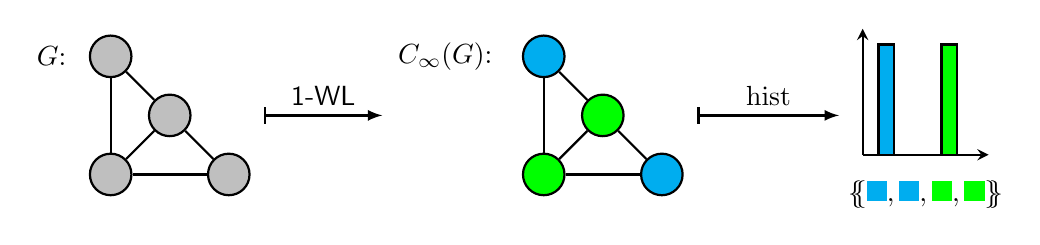
\begin{tikzpicture}
        \tikzset{line/.style={draw,thick}}
        \tikzset{arrow/.style={line,->,>=stealth}}
        \tikzset{node/.style={circle,inner sep=0pt,minimum width=15pt}}
        
        \draw (-1.5 - 1.5,0.75) node {$G$:};
        \node[line,node,fill=lightgray] (x1) at (-0.75 - 1.5, 0.75) {};
        \node[line,node,fill=lightgray] (x2) at (-0.75 - 1.5, -0.75) {};
        \node[line,node,fill=lightgray] (x3) at (0.75 - 1.5, -0.75) {};
        \node[line,node,fill=lightgray] (x4) at (0 - 1.5, 0) {};
        
        \path[line] (x1) to (x2);
        \path[line] (x1) to (x4);
        \path[line] (x2) to (x4);
        \path[line] (x3) to (x4);
        \path[line] (x2) to (x3);
    
        \draw [|-latex, thick] (1.2 - 1.5,0) -- node [text width=2.5cm,midway,above,align=center ] {$\wl$} (2.7 - 1.5,0);
        
        \draw (3.25 - 1.25, 0.75) node {$C_\infty(G)$:};
    
        \node[line,node,fill=cyan] (x1) at (-0.75 + 4.0, 0.75) {};
        \node[line,node,fill=green] (x2) at (-0.75 + 4.0, -0.75) {};
        \node[line,node,fill=cyan] (x3) at (0.75 + 4.0, -0.75) {};
        \node[line,node,fill=green] (x4) at (0 + 4.0, 0) {};
        
        \path[line] (x1) to (x2);
        \path[line] (x1) to (x4);
        \path[line] (x2) to (x4);
        \path[line] (x3) to (x4);
        \path[line] (x2) to (x3);
    
        \draw [|-latex, thick] (5.2,0) -- node [text width=2.5cm,midway,above,align=center ] {$\hist$} (6.7 + 0.3, 0);
        
        \filldraw[draw=black, fill=cyan, thick] (6.2 + 1.0+ 0.3, -0.5) rectangle (6.4 + 1.0+ 0.3, 0.9);
        \filldraw[draw=black!0, fill=orange!0, thick] (6.6 + 1.0+ 0.3, -0.5) rectangle (6.8 + 1.0+ 0.3, 0.2);
        \filldraw[draw=black, fill=green, thick] (7.0 + 1.0+ 0.3, -0.5) rectangle (7.2 + 1.0+ 0.3, 0.9);
    
        \draw[arrow, thick] (6.0 + 1.0+ 0.3, -0.5) to (7.6 + 1.0+ 0.3, -0.5);
        \draw[arrow, thick] (6.0 + 1.0+ 0.3, -0.5) to (6.0 + 1.0+ 0.3, 1.1);
    
        \draw (7.8+ 0.3, -1.0) node {$\MSopen \sqbox{cyan}, \sqbox{cyan}, \sqbox{green}, \sqbox{green} \MSclose$};
    
    
        \end{tikzpicture}    
\end{figure}

\begin{figure}[H]
    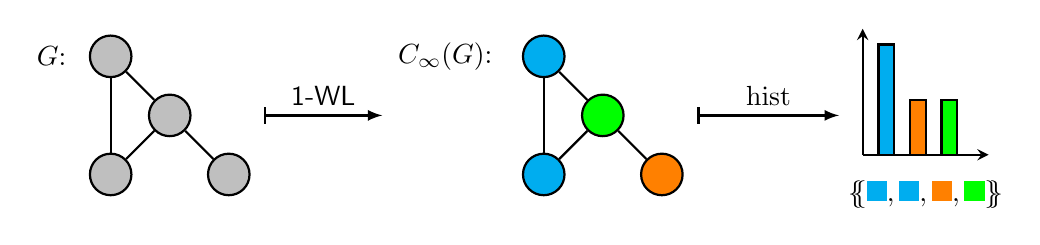
\begin{tikzpicture}
        \tikzset{line/.style={draw,thick}}
        \tikzset{arrow/.style={line,->,>=stealth}}
        \tikzset{node/.style={circle,inner sep=0pt,minimum width=15pt}}
        
        \draw (-1.5 - 1.5,0.75) node {$G$:};
        \node[line,node,fill=lightgray] (x1) at (-0.75 - 1.5, 0.75) {};
        \node[line,node,fill=lightgray] (x2) at (-0.75 - 1.5, -0.75) {};
        \node[line,node,fill=lightgray] (x3) at (0.75 - 1.5, -0.75) {};
        \node[line,node,fill=lightgray] (x4) at (0 - 1.5, 0) {};
        
        \path[line] (x1) to (x2);
        \path[line] (x1) to (x4);
        \path[line] (x2) to (x4);
        \path[line] (x3) to (x4);
    
        \draw [|-latex, thick] (1.2 - 1.5,0) -- node [text width=2.5cm,midway,above,align=center ] {$\wl$} (2.7 - 1.5,0);
        
        \draw (3.25 - 1.25, 0.75) node {$C_\infty(G)$:};
    
        \node[line,node,fill=cyan] (x1) at (-0.75 + 4.0, 0.75) {};
        \node[line,node,fill=cyan] (x2) at (-0.75 + 4.0, -0.75) {};
        \node[line,node,fill=orange] (x3) at (0.75 + 4.0, -0.75) {};
        \node[line,node,fill=green] (x4) at (0 + 4.0, 0) {};
        
        \path[line] (x1) to (x2);
        \path[line] (x1) to (x4);
        \path[line] (x2) to (x4);
        \path[line] (x3) to (x4);
    
        \draw [|-latex, thick] (5.2,0) -- node [text width=2.5cm,midway,above,align=center ] {$\hist$} (6.7 + 0.3, 0);
        
        \filldraw[draw=black, fill=cyan, thick] (6.2 + 1.0+ 0.3, -0.5) rectangle (6.4 + 1.0+ 0.3, 0.9);
        \filldraw[draw=black, fill=orange, thick] (6.6 + 1.0+ 0.3, -0.5) rectangle (6.8 + 1.0+ 0.3, 0.2);
        \filldraw[draw=black, fill=green, thick] (7.0 + 1.0+ 0.3, -0.5) rectangle (7.2 + 1.0+ 0.3, 0.2);
    
        \draw[arrow, thick] (6.0 + 1.0+ 0.3, -0.5) to (7.6 + 1.0+ 0.3, -0.5);
        \draw[arrow, thick] (6.0 + 1.0+ 0.3, -0.5) to (6.0 + 1.0+ 0.3, 1.1);
    
        \draw (7.8+ 0.3, -1.0) node {$\MSopen \sqbox{cyan}, \sqbox{cyan}, \sqbox{orange}, \sqbox{green} \MSclose$};
    
    
        \end{tikzpicture}    
\end{figure}

test \cite{Morris2018}

\setcitestyle{numbers}
\settocbibname{Bibliography}
\bibliography{references}


\end{document}